%%%%%%%%%%%%%%%%%%%%%%%%%%%%%%%%%%%%%%%%%%%%%%%%%%%%%%%%%%%%%%%
%
%
%   This file is included in Registration.tex
%
%   Lablels and section entries are defined in that file.
%
%
%
%%%%%%%%%%%%%%%%%%%%%%%%%%%%%%%%%%%%%%%%%%%%%%%%%%%%%%%%%%%%%%%

\itkpiccaption[Model to Image Registration Framework Components]{The basic components of model based registration are an image, a spatial object, a transform, a metric, an interpolator and an optimizer.\label{fig:ModelToImageRegistrationComponentsDiagram}}
\parpic(8cm,3.5cm)[r]{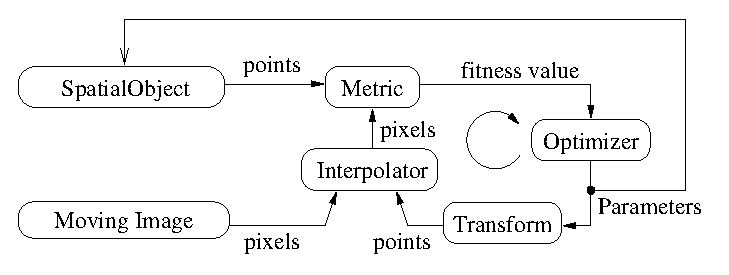
\includegraphics[width=7.5cm]{ModelToImageRegistrationComponentsDiagram.eps}}

This section introduces the concept of registering a geometrical model with
an image. We refer to this concept as \emph{model based registration} but
this may not be the most widespread terminology. In this approach, a
geometrical model is built first and a number of parameters are identified in
the model. Variations of these parameters make it possible to adapt the model
to the morphology of a particular patient. The task of registration
is then to find the optimal combination of model parameters that will
make this model a good representation of the anatomical structures
contained in an image.

For example, let's say that in the axial view of a brain image we can roughly
approximate the skull with an ellipse. The ellipse becomes our simplified
geometrical model, and registration is the task of finding the best center for
the ellipse, the measures of its axis lengths and its orientation in the plane.
This is illustrated in Figure~\ref{fig:ModelToImageRegistrationConcept}.  If we
compare this aproach with the image-to-image registration problem, we can see
that the main difference here is that in addition to mapping the spatial
position of the model, we can also customize internal parameters that change
its shape.

Figure~\ref{fig:ModelToImageRegistrationComponentsDiagram} illustrates the
major components of the registration framework in ITK when a model base
registration problem is configured. The basic input data for the registration
is provided by pixel data in an Image and by geometrical data stored
in a SpatialObject. A metric has to be defined in order to evaluate
the fitness between the model and the image. This fitness value can be improved
by introducing variations in the spatial positioning of the
SpatialObject and/or by changing its internal parameters. The search
space for the optimizer is now the composition of the transform parameter and
the shape internal parameters.

This same approach can be considered a segmentation technique, since once the
model has been optimally superimposed on the image we could label pixels
according to their associations with specific parts of the model. The
applications of model to image registration/segmentation are endless.  
The main advantage of this approach is probably that, as opposed to image-to-image
registration, it actually provides \emph{Insight} into the anatomical structure
contained in the image. The adapted model becomes a condensed representation of
the essential elements of the anatomical structure.

\begin{figure}
\center
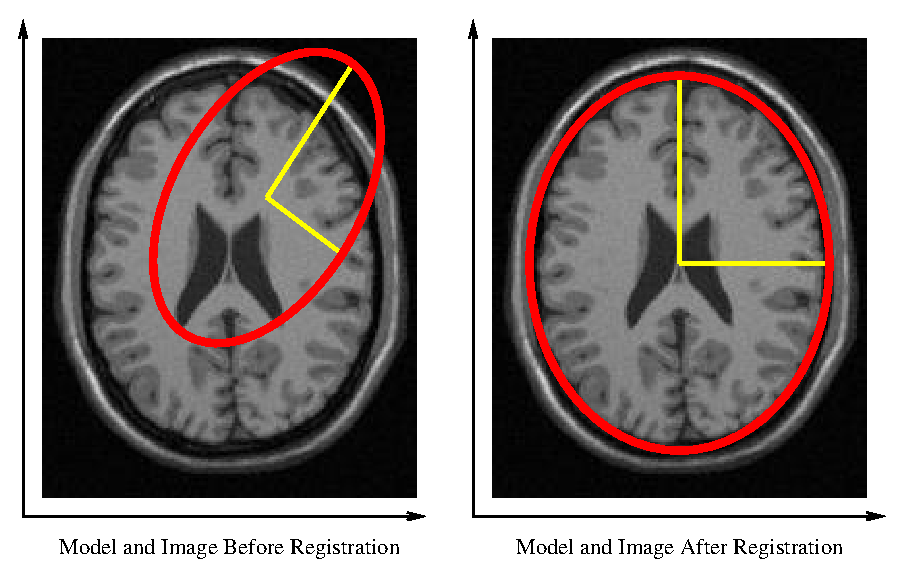
\includegraphics[width=0.8\textwidth]{ModelToImageRegistrationConcept.eps}
\itkcaption[Model to Image Registration Framework Concept]{Basic concept of
  Model-to-Image registration.  A simplified geometrical model (ellipse) is
    registered against an anatomical structure (skull)  by applying a spatial
    transform and modifying the model internal parameters. This image is not
    the result of an actual registration, it is shown here only with the
    purpose of illustrating the concept of model to image registration.}
\label{fig:ModelToImageRegistrationConcept}
\end{figure}


ITK provides a hierarchy of classes intended to support the construction of
shape models. This hierarchy has the SpatialObject as its base class.
A number of basic functionalities are defined at this level, including the
capacity to evaluate whether a given point is \emph{inside} or \emph{outside} of the
model, form complex shapes by creating hierarchical
conglomerates of basic shapes, and support basic spatial
parameterizations like scale, orientation and position.

The following sections present examples of the typical uses of these powerful
elements of the toolkit.

%\ifitkFullVersion
\input{ModelToImageRegistration1.tex} 
%\fi




